\section{Fundamentos de Bolsa}
	
		\subsection{Mercado de valores}
		
		El mercado de valores o bolsa es un tipo de mercado en el que se compran y venden productos burs\'atiles. Para este trabajo, prestaremos principal atenci\'on a las acciones, el producto burs\'atil m\'as simple de un mercado de valores.\\
		
		Una acci\'on equivale a una pequeña participaci\'on en la empresa a la que pertenece la acci\'on. De esta forma, inversores privados tienen la posibilidad de comprar porciones de empresas. Por ejemplo, si una empresa est\'a dividida en 200 acciones, tras comprar 50 de estas, ser\'iamos propietarios de una cuarta parte de la empresa. Ser part\'icipes del accionariado de una empresa puede reportarnos beneficios de distinta \'indole seg\'un las normas de la misma. En ocasiones algunas empresas deciden repartir una determinada cantidad de dinero entre sus accionistas a partir de las ganancias obtenidas en un periodo (dividendo). Otras veces, ser poseedor de una gran parte de la empresa otorgar\'a derechos dentro de la misma como, por ejemplo, participar en las decisiones importantes que se tomen.\\
		
		Por \'ultimo, el mercado de valores espa\~nol abre de 9:00 a 17:30 de lunes a viernes. Pero cabe destacar que hay una aleatoriedad de 30 segundos, es decir, la hora exacta de la apertura y del cierre var\'ia de forma no definida hasta en 30 segundos. Además, despu\'es del cierre hay un periodo de subasta de 5 minutos, durante el cual el valor de las acciones est\'a oculto para evitar manipulaciones de los precios en los \'ultimos minutos. No obstante, no es el momento de explicar a fondo el funcionamiento interno de un mercado de valores. Nos ser\'a suficiente con los puntos b\'asicos anteriormente explicados.\\
		
		\subsection{El valor de las acciones}
		
		El valor de una acci\'on no es fijo, si no que cambia seg\'un la oferta y la demanda de las acciones de la empresa. Esto convierte a las acciones en un producto muy conveniente para especular.\\
		
		El mecanismo de compra y venta es el que define el valor de una acci\'on. Para comprar o vender, un inversor debe enviar a bolsa una orden de compra o venta, respectivamente. Tras enviar la orden, esta queda registrada y esta ser\'a ejecutada tan pronto como sea posible. Aclaremos este proceso con un ejemplo sencillo:\\
		
		Supongamos que existe una empresa que tiene en el mercado cuatro acciones. Cada una de ellas pertenece a un propietario distinto, llamados A, B, C y D. \\
		
		El inversor A tiene una orden de venta de su acci\'on a 4 euros y C tiene una orden de compra de una acci\'on a 1 euro. En esta situaci\'on ninguno puede vender ni comprar, y el precio queda situado en 4 euros por acci\'on. Ahora bien, el accionista B decide vender su acci\'on por 3 euros. En el momento en el que realiza una orden de venta, el precio de las acciones baja a 3 euros. Esto no quiere decir que el inversor A venda su acci\'on a este precio. Para bajar de 4 a 3 euros el precio de su acci\'on deber\'ia cancelar la orden y realizar una nueva. En esta situaci\'on no se puede ejecutar ninguna orden en el mercado, como se puede ver en la figura \ref{fig:ordenes_ejemplo}.\\
		
				\begin{figure}[H]
					\centering
					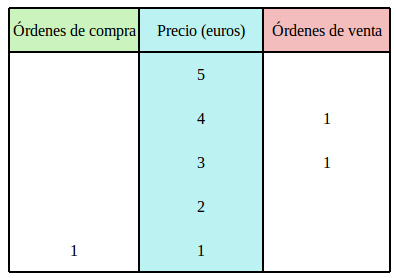
\includegraphics[scale=2]{imagenes/ordenes_ejemplo.png}
					\caption[Ejemplo de situaci\'on de las \'ordenes]{Situaci\'on de las \'ordenes.\\ Fuente: elaboraci\'on propia.}
					\label{fig:ordenes_ejemplo}
				\end{figure}
		
		
		De este modo, tras conocer que el precio de la acci\'on ha bajado de 4 a 3 euros, el inversor D decide comprar y sit\'ua una orden de compra a 3 euros de una acci\'on. Entonces, la orden de venta de C y la orden de compra de D pueden ejecutarse y, por ende, anularse. Ahora el inversor D pasa a tener 2 acciones y el mercado se queda con tan solo las dos \'ordenes de A y B. A causa de este hecho, el precio de la acci\'on vuelva a subir a 4 euros, la orden de venta m\'as baja.\\
		
		En el ejemplo anterior se han simplificado las \'ordenes de compra y venta. En realidad, las ordenes que existen son un poco m\'as complejas:\\
		
		\begin{itemize}
			
			\item \textbf{Orden de mercado.} Con este tipo de orden se compran todas las acciones que se especifiquen al mejor precio posible. En caso de que la orden sea de compra, se adquieren acciones a los precios m\'as bajos, en caso de que sea de venta, a los precios m\'as altos. Refiriendo al caso anterior, si B hubiera emitido una orden de mercado de una acci\'on, habría comprado la acci\'on del inversor A, que en este caso ten\'ia un valor de 4 euros.
			
			\item \textbf{Orden limitada.} En este caso, se compran todas las acciones que se emitan en la orden siempre y cuando su precio est\'e situado en un l\'imite establecido. Por ejemplo, si D hubiera emitido una orden limitada a 3 euros de dos acciones, hubiera comprado por 3 euros la acci\'on de C pero no hubiera adquirido la de A, que estaba situada a 4 euros. La orden limitada permanece vigente hasta que la suma total de las acciones sea comprada.
			
			\item \textbf{Orden on Stop.} En esta modalidad, la orden no se hace efectiva hasta que el precio de las acciones llega al precio estipulado en la orden. Una vez llegado ese momento, la orden se convierte en una orden de mercado, es decir, se compran o se venden todas las acciones que se especifiquen en la misma al mejor precio posible.
			
			\item \textbf{Orden Stop-Limit.} Este tipo de orden no se hace efectiva hasta que el precio de las acciones no llegue al precio de la orden. En ese momento, la orden se convierte en una orden limitada. Es muy frecuente que las plataformas ofrezcan este tipo de orden, pues funciona como seguro para no perder todo el capital cuando las acciones caen de precio r\'apidamente. Si se sospecha que las acciones pueden bajar su valor, se coloca una orden stop-limit de venta a un precio que se considere bajo. De este modo, si el valor de las acciones decae, estas se venden de forma autom\'atica. 
			
		\end{itemize} 
		
		\subsection{Corredores de bolsa o brokers}
	
		Para agilizar las transacciones en bolsa, no se permite que particulares env\'ien \'ordenes al mercado. Esta tarea se delega en los corredores de bolsa o \textit{brokers}. La entidad de \textit{broker} se encarga de captar inversores, lanzar \'ordenes a bolsa y presentar a compradores con vendedores. Para ser broker se debe aprobar un examen y demostrar que se tienen los conocimientos necesarios. A cambio de realizar este trabajo se lleva una comisi\'on que todo inversor debe abonar. \\
		
		Las comisiones pueden ser de dos tipos:\\
		
		\begin{itemize}
			\item \textbf{Comisiones fijas.} Son un valor fijo que cada broker cobra. Pueden ser por transacci\'on, seg\'un cantidad de acciones y su precio, y por tiempo de servicio, seg\'un la cantidad de d\'ias que el cliente dispone para realizar transacciones. Las comisiones fijas son beneficiosas para inversores con un gran capital.
			
			\item \textbf{Comisiones variables.} Son precios variables que dependen del país de inversión, la cantidad invertida e incluso el tiempo que dura una inversi\'on. Las comisiones variables afectan en la misma medida a inversores grandes y peque\~nos. Por este motivo, un inversor con poco capital pagar\'a menos comisiones con este tipo de cobro.
		\end{itemize}
		
		La mayor\'ia de los corredores de bolsa tienen comisiones mixtas. Algunos cobran distintas comisiones seg\'un la bolsa en la que se quiera operar. \\
		
		Sirva todo lo anteriormente expuesto como introducci\'on a los mecanismos y herramientas que intervienen en el mercado de valores. Solo debemos a\~nadir que en los supuestos que trabajaremos m\'as adelante, utilizaremos una comisiones variable del 1\% de la cantidad invertida. Esto implicar\'a que por cada 100 euros invertidos, se perder\'a 1 en concepto de comisiones de \textit{broker}.\\
